\documentclass[a4paper, 11pt, titlepage]{article}
\usepackage{fancyhdr}
\usepackage{graphicx}
\usepackage{imakeidx}
\usepackage{makeidx}
\usepackage{mathtools}
\usepackage[spanish]{babel}
\usepackage{eurosym}
\usepackage{hyperref}
\usepackage{amssymb}
\usepackage{listings}
\usepackage{xcolor}
\usepackage{subcaption}

\setcounter{secnumdepth}{5}
\setcounter{tocdepth}{5}

\title{{\scshape\Huge Sistemas Operativos Distribuidos \par}}
\author{Francisco Javier Balón Aguilar}

\begin{document}
\maketitle
\renewcommand{\contentsname}{Índice de contenidos} % Nombre dado al ?ndice
\tableofcontents % Genera la tabla de contenidos del ?ndice autom?ticamente
%\newpage

%Lista de figuras 
\listoffigures
%\newpage

%Lista de tablas 
\listoftables
\newpage

% \section{Introducción}
%     \subsection{Estructura de un sistema distribuido}
%         \subsubsection{Funciones de un sistema distribuido}
%         \subsubsection{Características de un sistema distribuido}
%     \subsection{Tipos de sistemas operativos distribuidos}

\section{Sistemas operativos multiprocesador}

    \subsection{Arquitectura de un sistema operativo multiprocesador}

        Los equipos que cuentan con más de un procesador y que comparten la misma memoria
        se denominan sistemas multiprocesador. En ellos, debe existir un sistema operativo 
        común y central, que controle las operaciones de cada procesador, así como su 
        gestión, coordinación y accesos a memoria.

        Este tipo de sistemas proporcionan una mayor productividad del sistema, ya que 
        pueden realizar un mayor número de tareas en un menor espacio de tiempo, y una 
        mayor velocidad de aplicación, ya que al aumentarse el número de procesadores,
        disminuye el tiempo de espera de un proceso para ser procesado.

        Estos sistemas ofrecen una serie de ventajas:

        \begin{itemize}
            \item \textbf{Rendimiento y potencia de cálculo}.
            \item \textbf{Tolerancia a fallos}.
            \item \textbf{Flexibilidad}.
            \item \textbf{Relación coste/rendimiento}.
        \end{itemize}

        Podemos clasificar los sistemas multiprocesador según el modo de trabajo en:

        \begin{itemize}
            \item \textbf{Procesamiento asimétrico}
            
            El procesamiento asimétrico\footnote{
                El modo de procesamiento asimétrico se originó en 1970 en el Instituto
                 Tecnológico de Massachusetts (M.I.T.). 
            } entre varios ordenadores permite ejecutar procesos 
            de manera independiente separados del procesador que controla y tiene instalado
            el sistema operativo.\footnote{
                A día de hoy este modo de procesamiento no se utiliza casi salvo en 
                aplicaciones muy concretas como puede ser la PS3 de Sony, donde el 
                procesador central tiene sub-procesadores que se encargan de tareas 
                muy específicas.
            }

            Aunque a nivel físico ya no se utilice este diseño de arquitectura, a nivel 
            lógico si que se sigue implantando en sistemas donde cada procesador se encarga
            de una tarea específica, por ejemplo, un procesador puede ser el responsable
            de las operaciones de disco, otro de las operaciones de video, etc. Estos
            sistemas no tienen la flexibilidad de asignación de tareas a los procesadores 
            menos cargados, estando predefinidas por defecto.

            \begin{figure}[htp]
                \centering
                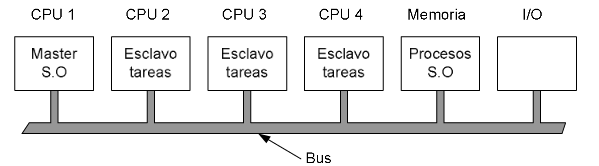
\includegraphics[width=1\textwidth]{resources/multiprocesador_asimetrico.png}
                \caption{Representación de multiprocesador asimétrico}
                \label{multiprocesador_asimetrico}
            \end{figure}

            \item \textbf{Procesamiento simétrico}
            
            En un sistema multiproceso, cada uno de los procesadores deben ser equivalentes,
            con funciones similares, aunque haya alguno que realice tareas específicas.

            A nivel de hardware, en los sistemas simétricos cada procesador puede acceder a 
            la memoria RAM por completo. Cada procesador tiene la misma importancia a la hora
            de acceder, por lo tanto todas las CPUs pueden interaccionar y compartir memoria 
            entre ellas.
            
            A nivel de software, e independientemente del sistema operativo que lo gestione, 
            cada procesador tiene capacidad para enviar o repartir tareas a otros procesadores. 
            Al no existir una unidad central, y tener acceso total a la memoria, cada procesador 
            es capaz de terminar cualquiera de las tareas asignadas. \footnote{
                Al ser todos los procesadores idénticos, ante el fallo de uno de ellos el sistema 
                operativo lo retira y lo notifica al operador. Todos los procesadores pueden cooperar
                en la ejecución de un mismo proceso. Aun así, esta arquitectura también puede producir 
                largas colas de espera.
            }

            \begin{figure}[htp]
                \centering
                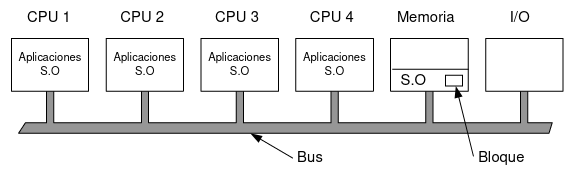
\includegraphics[width=1\textwidth]{resources/multiprocesador_simetrico.png}
                \caption{Representación de multiprocesador simétrico}
                \label{multiprocesador_simetrico}
            \end{figure}
        \end{itemize}

        Podemos clasificarlos también según el modo de ejecución de instrucciones, atendiendo al 
        número de instrucciones y datos que son capaces de procesar a la vez (véase cuadro 
        \ref{modoejecucioninstrucciones}):

        \begin{table}[htp]
            \centering
            \caption{Modos de ejecución de instrucciones}
            \label{modoejecucioninstrucciones}
            \begin{tabular}{rcc}
                %\hline
                & \textbf{Un dato} & \textbf{Múltiples datos} \\ \hline
                \textbf{Una instrucción} & SISD & SIMD \\ \hline
                \textbf{Múltiples instrucciones} & MISD & MIMD \\ \hline
            \end{tabular}
        \end{table}

        \begin{itemize}
            \item \textbf{Sistemas SISD} (Single  Instruction  Stream,  Single  Data  Stream). Un 
            procesador procesa secuencialmente instrucciones, y cada instrucción lleva un dato asociado; 
            siendo los sistemas menos efectivos.
            \item \textbf{Sistemas SIMD} (Single  Instruction  Stream,  Multiple  Data  Stream). 
            El procesador ejecuta una instrucción que puede llevar asociada varios datos.
            \item \textbf{Sistemas MISD} (Multiple  Instruction  stream,  Single  Data  stream). Tienen  
            como ventaja fundamental la tolerancia a los fallos. La redundancia de varias unidades de
            proceso trabajando sobre los mismos datos aumenta la fiabilidad del sistema, ya que el fallo 
            de una de las unidades de proceso no supondría ningún inconveniente. Por otro lado, estos 
            sistemas encarecen demasiado la arquitectura y no aumentan el rendimiento ni la velocidad de 
            proceso. 
            \item \textbf{Sistemas MIMD} (Multiple Instruction stream, Multiple Data stream). Este tipo 
            de arquitectura es el más adecuado para una enorme variedad de tareas en las que se desarrollan 
            ejecuciones independientes en paralelo utilizando conjuntos de datos independientes. 

            El procesamiento y ejecución se divide en lo que se llaman hilos, cada uno con su propio 
            procesador, y pertenecientes a uno o varios procesos software. Desde este punto de vista se
            deben controlar bloqueos que se puedan producir por la interferencia de varios hilos a los 
            mismos recursos, como por ejemplo la memoria.

            A nivel de hardware es una arquitectura fácil de implementar, aunque a nivel software se debe
            controlar el acceso compartido con mecanismos como semáforos que eviten los bloqueos mutuos 
            entre procesos. 

            Dentro de esta arquitectura, el procesador y la memoria pueden presentar dos esquemas según 
            estén conectados:
            
            \begin{itemize}
                \item \textbf{Modelos  fuertemente  acoplados}. Los procesadores comparten memoria entre sí,
                lo que puede provocar que en determinadas ocasiones se produzcan bloqueos de acceso.
                Dentro del tipo de acceso a memoria, existen dos tipos:
                
                \begin{itemize}
                    \item \textbf{UMA} o acceso uniforme a memoria.
                    \item \textbf{NUMA} o acceso no uniforme a memoria, donde  la  velocidad  de acceso a 
                    distintas zonas de memoria puede ser distinta.
                \end{itemize}

                Véase figura \ref{modelo_fuertemente_acoplado} para más detalle.
        
                \item \textbf{Modelos   débilmente   acoplados}. Cada procesador gestiona su propia 
                memoria, teniendo como norma el acceso no remoto a memoria (siendo local). Véase figura 
                \ref{modelo_debilmente_acoplado} para más detalle.
            \end{itemize}

            \begin{figure}[!tbp]
                \begin{subfigure}[b]{0.5\textwidth}
                  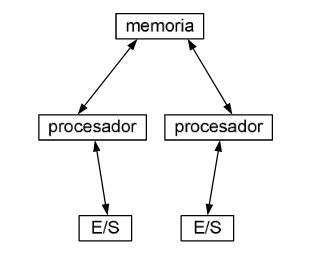
\includegraphics[width=\textwidth, height=\textwidth]{resources/modelo_fuertemente_acoplado_mimd.png}
                  \caption{Modelo fuertemente acoplado}
                  \label{modelo_fuertemente_acoplado}
                \end{subfigure}
                \hfill
                \begin{subfigure}[b]{0.5\textwidth}
                  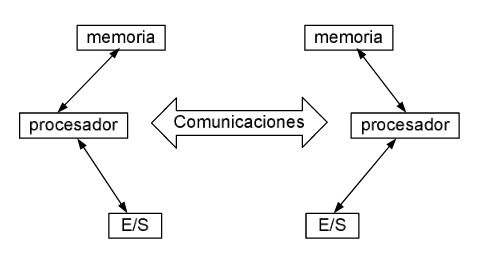
\includegraphics[width=\textwidth, height=\textwidth]{resources/modelo_debilmente_acoplado_mimd.png}
                  \caption{Modelo débilmente acoplado}
                  \label{modelo_debilmente_acoplado}
                \end{subfigure}
                \caption{Modelos de acoplamiento sobre arquitectura MIMD}
              \end{figure}
        \end{itemize}

        \subsubsection{Interconexión de los procesadores}

            El modo en el que los procesadores están conectados es fundamental para el rendimiento
            y velocidad del sistema. Existen diversos modos, pero los cuatro fundamentales son:

            \begin{enumerate}
                \item \textbf{Conexión con bus compartido}. Todos los procesadores están conexionados por el mismo 
                bus, lo que hace que desde el nivel lógico del sistema operativo no sea lo más eficiente, además 
                de dependiente de la velocidad que soporte el propio bus. Véase figura \ref{bus_compartido}.

                \begin{figure}[htp]
                    \centering
                    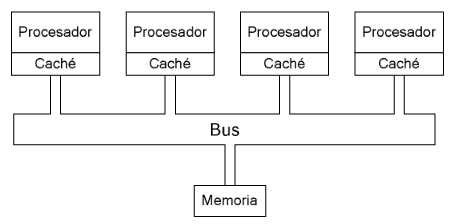
\includegraphics[width=0.7\textwidth]{resources/bus_compartido.png}
                    \caption{Conexión con bus compartido}
                    \label{bus_compartido}
                \end{figure}
    
                \item \textbf{Sistema de barras cruzadas}. Todos los procesadores pueden acceder a todas las 
                memorias simultáneamente, siendo el único retardo la conmutación de barras y haciendo este tipo 
                de conexión más eficiente que la anterior. Aun así, es una arquitectura compleja que necesita 
                $n^2$ conmutadores. Véase figura \ref{barras_cruzadas}.

                \begin{figure}[htp]
                    \centering
                    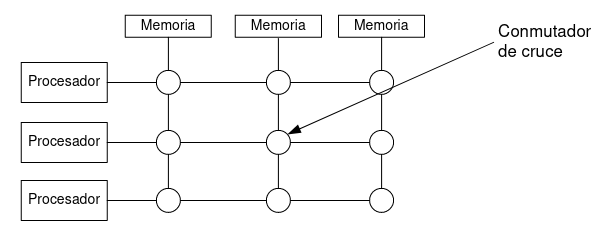
\includegraphics[width=0.8\textwidth]{resources/barras_cruzadas.png}
                    \caption{Conexión con barras cruzadas}
                    \label{barras_cruzadas}
                \end{figure}

                \item \textbf{Conexión mediante hipercubos}. Los procesadores y las memorias se conectan 
                formando hipercubos, siendo la máxima distancia entre nodos $log_2n$ y cada nodo a su vez 
                se conecta con $log_2n$ nodos (cada hipercubo contiene hipercubos de menor dimensión). Esto 
                lo convierte en un modelo complejo pero escalable (complejidad con crecimiento logarítmico, 
                no exponencial). Véase figura \ref{hipercubos}.
                
                \begin{figure}[htp]
                    \centering
                    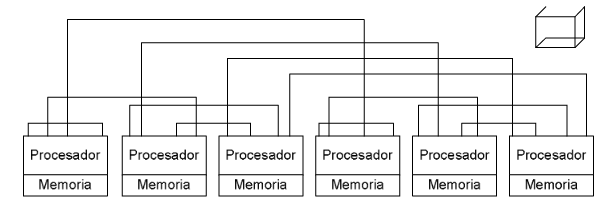
\includegraphics[width=0.8\textwidth]{resources/hipercubos.png}
                    \caption{Conexión mediante hipercubos}
                    \label{hipercubos}
                \end{figure}

                \item \textbf{Conexión mediante conmutadores multietapa}. Está formado por $log_2n$ etapas, 
                donde cada etapa consta de un conjunto de $n$ enlaces conectando a $n/2$ cajas de intercambio.
                Esto lo convierte en un modelo complejo pero escalable (complejidad con crecimiento logarítmico, 
                no exponencial). Véase figura \ref{conmutadores_multietapa}.
                
                \begin{figure}[htp]
                    \centering
                    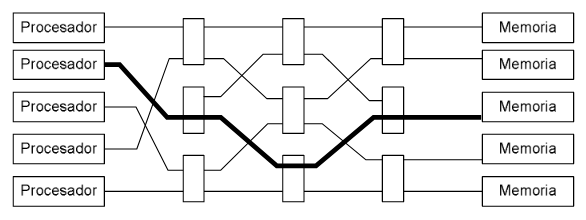
\includegraphics[width=0.8\textwidth]{resources/conmutadores_multietapa.png}
                    \caption{Conexión mediante conmutadores multietapa}
                    \label{conmutadores_multietapa}
                \end{figure}

            \end{enumerate}

    \subsection{Gestión del procesador}

        Para garantizar el correcto funcionamiento de un procesador, se desarrollan operaciones de control y
        gestión. Al existir varios procesadores dentro de una misma máquina, deben actuar y coordinarse como
        un solo procesador virtual.

        \subsubsection{Asignación de los procesadores}

            Dentro de los procesadores del sistema, un procesador puede ser a la vez gestor y trabajador:
            
            \paragraph{Procesador como gestor} Se crea una jerarquía de niveles en la que cada procesador 
            depende de los procesadores situados en un nivel superior. De este modo un procesador recibe 
            órdenes de los procesadores situados en niveles superiores, y asigna trabajos a los 
            procesadores inactivos situados en niveles inferiores. De esta forma se dota al sistma de una 
            mayor tolerancia a fallos.  

            \paragraph{Planificación por oleadas} Un gestor generalmente recibe órdenes que debe repartir 
            a lo largo de la jerarquía. Si puede asignar el trabajo a alguno de los procesadores que están 
            por debajo de él, lo hace, si no trata de ejecutar él el trabajo, y en caso de que no sea 
            posible, lo pasa a niveles superiores. Si llega a la máxima jerarquía y ha sido incapaz de 
            asignarlo, el trabajo se queda en espera pendiente de asignación hasta que haya algún procesador 
            libre.

            \paragraph{Problemas y dificultades} El gestor debe saber cuándo un procesador queda libre de 
            asignación, por lo que debe tener una estimación actualizada de la disponibilidad de cada 
            procesador en cada momento para evitar repartos de carga erróneos.

        \subsubsection{Planificación del procesador}

            Según la política de planificación del sistema, cada procesador puede estar monoprogramado\footnote{
                Las tareas que le han sido asignadas son independientes del resto de los procesadores, es decir, no trabaja  en  cooperación  con  ningún  procesador  más.
            }
            o multiprogramado\footnote{
                La ejecución de tareas asignadas se produce en cooperación con varios procesadores entre sí.
            }.

            \paragraph{Tipos de planificación}

                Dependiendo del tipo de instrucciones y del tipo de arquitectura, el sistema se puede 
                decantar por distintos modos de ejecución:

                \subparagraph{Coplanificación}

                    Existe una coplanificación o planificación coordinada entre los procesos que 
                    interactúan para que se ejecuten al mismo tiempo.

                \subparagraph{Compartición de cargas}

                    Se crea una cola global de hilos (tareas) para todos los procesadores, de tal forma que 
                    elimina la necesidad de que las tareas estén asignadas a un mismo proceso.

                \subparagraph{Asignación dedicada de procesadores}

                    Pretende ejecutar un proceso lo antes posible, por lo que se divide el proceso en 
                    hilos o tareas, y se asigna un procesador (distinto) a cada hilo, es decir, a cada
                    proceso se le asignan tantos procesadores como hilos tenga. 

                \subparagraph{Planificación dinámica}

                    Se permite cambiar el número de hilos de un proceso para permitir ajustar la carga al
                    sistema operativo, permitiendo la expulsión de algún proceso en curso y haciendo que éste 
                    sea el tipo de planificación más utilizado.

            \paragraph{Algoritmos de planificación}

                \subparagraph{Algoritmo de tiempo compartido}

                    Logra equilibrar la carga de tareas entre todos los procesadores de un sistema 
                    distribuyendo las tareas de forma equilibrada, utilizando una estructura de datos 
                    simple para la planificación y siendo todos los procesos de tiempo compartido, evitando 
                    así sobrecargas en el sistema. Véase figura \ref{algoritmo_tiempo_compartido}.

                    \begin{figure}[htp]
                        \centering
                        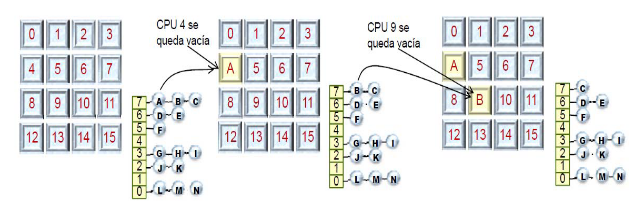
\includegraphics[width=0.8\textwidth]{resources/algoritmo_tiempo_compartido.png}
                        \caption{Representación de algoritmo de tiempo compartido}
                        \label{algoritmo_tiempo_compartido}
                    \end{figure}

                \subparagraph{Algoritmo de espacio compartido}

                    Divide el conjunto de procesadores en grupos que ejecutarán tareas similares, utilizando 
                    coplanificación o planificación coordinada entre procesos para que se ejecuten al mismo tiempo.

                    Las particiones de grupos se basan en hilos relacionados\footnote{
                        La planificación de varios hilos relacionados al mismo tiempo sobre múltiples CPU’s se 
                        llama space sharing. 
                    }, de tal forma que cada conjunto 
                    de procesadores asociados como grupo ejecute una parte completa de un proceso. A cada hilo 
                    en un grupo se le asigna una CPU dedicada hasta que termine\footnote{
                        Si un hilo realiza una operación de entrada y salida y se bloqueara, continuaría ocupando 
                        la CPU, pudiendo dar un bloqueo indefinido.
                    }.

                    Como ejemplo, si tuviéramos un conjunto de 32 procesadores divididos en cuatro particiones con 
                    dos procesadores sin asignar, tendríamos un mapa de utilización tal y como aparece en la figura 
                    \ref{algoritmo_espacio_compartido}.

                    \begin{figure}[htp]
                        \centering
                        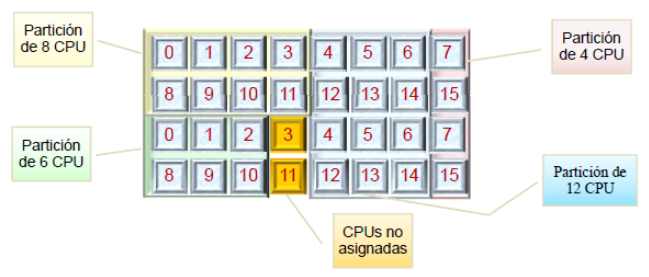
\includegraphics[width=0.8\textwidth]{resources/algoritmo_espacio_compartido.png}
                        \caption{Representación de algoritmo de espacio compartido}
                        \label{algoritmo_espacio_compartido}
                    \end{figure}

                \subparagraph{Algoritmo de planificación por grupos}

                    Planificando como una sola unidad de conjuntos de hilos que por su funcionalidad se relacionan 
                    entre sí (\textit{gang}), todos los miembros de un grupo se ejecutan simultáneamente en diferentes 
                    procesadores de tiempo compartido; diviendo el tiempo en \textit{quantums}\footnote{
                        Los quantums no son una medida estándar de tiempo, depende del sistema y puede establecerse
                        como un número determinado de ciclos de procesador. 
                    }, de tal forma que todos los miembros del grupo comiencen y terminen sus \textit{quantums} juntos.
               
                    Al comienzo de un \textit{quantum} se replanifican todos los procesadores con un nuevo hilo 
                    en cada uno de ellos. Al comienzo del siguiente se realiza otra planificación independiente de la 
                    primera. Cabe destacar que si un hilo se bloquea, el procesador permanecerá inactivo hasta el 
                    final del \textit{quantum}.

                    Como ejemplo, si tuviéramos una planificación por grupos con 6 procesadores, 5 procesos y 24 hilos, 
                    todos los hilos de un proceso se ejecutarán juntos, por lo que si uno de ellos envía una petición 
                    a otro, éste recibirá el mensaje y lo contestará inmediatamente. Véase figura \ref{algoritmo_planificacion_grupos}.

                    \begin{figure}[htp]
                        \centering
                        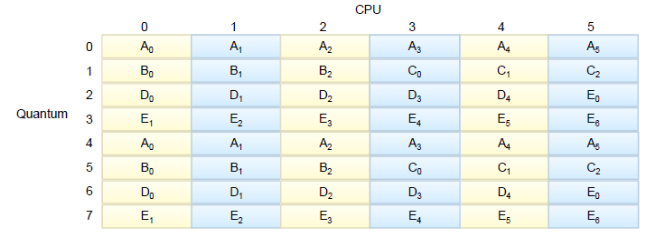
\includegraphics[width=0.8\textwidth]{resources/algoritmo_planificacion_grupos.png}
                        \caption{Representación de ejecución de algoritmo de planificación por grupos}
                        \label{algoritmo_planificacion_grupos}
                    \end{figure}
                
                    Las comunicaciones entre dos hilos lleva un retardo asociado debido a la gestión de los mensajes.
    
                    Como ejemplo, si el proceso $A$ tiene dos hilos, $A_0$ y $A_1$, y el proceso $B$ tiene otros dos hilos,
                    $B_0$ y $B_1$, y $A_0$ y $B_0$ se ejecutan en el procesador 0, y $A_1$ y $B_1$ en el procesador 1:

                    \begin{itemize}
                        \item $A_0$ envía un mensaje a $A_1$, y $A_1$ envía la respuesta nada más recibir el mensaje.
                        \item $A_0$ envía el mensaje, pero recibe la respuesta con un retardo de $200ms$ debido a los hilos de $B$.
                    \end{itemize}

                    Véase figura \ref{esquema_comunicacion_dos_hilos}.

                    \begin{figure}[htp]
                        \centering
                        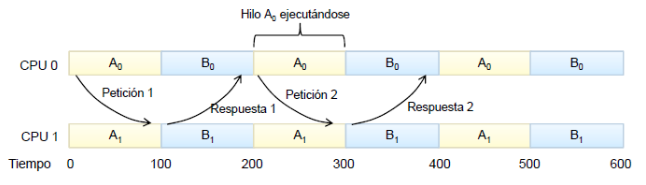
\includegraphics[width=0.8\textwidth]{resources/esquema_comunicacion_dos_hilos.png}
                        \caption{Esquema de comunicación entre dos hilos}
                        \label{esquema_comunicacion_dos_hilos}
                    \end{figure}

    \subsection{Sincronización y gestión de la memoria}

        La sincronización es el proceso por el cual diferentes aplicaciones y procesadores pueden acceder 
        a la memoria de manera ordenada y sin interferir en la lectura o escritura de datos.

        Para acceder a una zona compartida de memoria, se deben ejecutar tres pasos básicos:

        \begin{itemize}
            \item Bloquear el bus para que las otras CPU’s no puedan acceder a él (lock).
            \item Ejecuta la instrucción TSL\footnote{
                De hecho la instrucción TSL puede fallar en algunas ocasiones, por ejemplo si el bus no 
                está bloqueado, lo que puede generar algún acceso no controlado a memoria.
            } (Test and Set Lock) para bloquear el bus. 
            \item Desbloquear el bus.
        \end{itemize}

        Estos pasos se pueden ejecutar preferiblemente por hardware, o por medio de la instrucción
        software lock.

        \begin{figure}[htp]
            \centering
            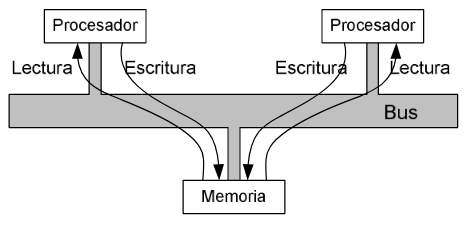
\includegraphics[width=0.5\textwidth]{resources/interaccion_procesadores_memoria_bus.png}
            \caption{Interacción de procesadores y memoria a través del bus}
            \label{interaccion_procesadores_memoria_bus}
        \end{figure}

        Cuando un procesador libera la memoria, debe avisar a aquellos procesos que se hayan quedado 
        esperando para entrar. Este proceso de espera activa por parte de las CPU’s que no hayan podido 
        entrar se llama spinning, y es el proceso por el cual un procesador se encuentra bloqueado 
        (lock) con un trabajo pendiente para entrar en zona de memoria compartida. Véase la figura 
        \ref{bloqueo_espera_activa_spin}.

        \begin{figure}[htp]
            \centering
            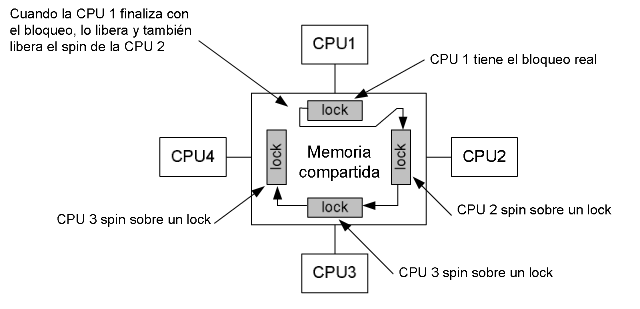
\includegraphics[width=0.8\textwidth]{resources/bloqueo_espera_activa_spin.png}
            \caption{Mecanismo de bloqueo con espera activa (spin)}
            \label{bloqueo_espera_activa_spin}
        \end{figure}

        \subsubsection{Algoritmos de sincronización}

            \paragraph{Algoritmo de sincronización a través de átomos}

                Un átomo se define como un objeto accesible (se puede leer y escribir) con la propiedad 
                de que sólo puede ser accedido a la vez por un procesador. 

                Para controlar el acceso de los procesadores a los átomos, se suele implementar un 
                algoritmo de sincronización específico para este tipo de objetos:

                \subparagraph{Sincronización por cerrojo}

                    Existe un elemento que indica si el átomo está ocupado o está libre, de tal manera 
                    que el proceso que accede al átomo bloquea el cerrojo (o lo cierra), y no lo abre 
                    hasta que no ha terminado sus operaciones en el átomo. 

                \subparagraph{Sincronización optimista}

                    El átomo mantiene dos versiones de la información, una local y otra global. El proceso 
                    que accede al átomo modifica la versión local del mismo. Una vez ha terminado, 
                    actualiza la versión global. El resto de procesos pueden acceder a la versión 
                    global del átomo (para leer información). Este método puede provocar inconsistencia 
                    en los datos.

                \subparagraph{Sincronización por servidor}
                
                    Se controla el acceso a los átomos de forma centralizada desde un servidor designado.

            \paragraph{Protocolos de espera}

                Existen dos tipos de espera dentro del procesador:

                    \subparagraph{Espera ocupada}

                        Cuando un proceso no puede acceder a un átomo, el proceso sigue ocupando el 
                        procesador, esperando a que ese átomo que solicita sea liberado.
            
                        Existe lo que se llama el protocolo de servicio completo, donde se notifica 
                        la liberación de un átomo a todos los procesadores (independientemente que 
                        quieran acceder o no).

                    \subparagraph{Espera suspendida}

                        El procesador <<echa>> al proceso que no puede acceder al átomo en ese momento, 
                        metiéndolo en una cola de espera. Este método puede generar cuellos de botella 
                        si el acceso a los átomos es muy prolongado por parte de algunos procesos.

\section{Servicios de tiempo}

    Este capítulo pretende introducir el concepto de gestión del tiempo dentro de un sistema distribuido, 
    tanto a nivel físico, como lógico; siendo el tiempo un factor fundamental en todo sistema distribuido
    \footnote{
        Un ejemplo de sincronización de eventos son las transacciones, donde es fundamental saber el 
        tiempo en el que se ha ejecutado una acción para poder establecer un orden entre ellas y que no 
        se produzcan errores. 
    }.

    Existen varios tipos de sincronización temporal, de entre las que destacan la sincroniación externa 
    (cada máquina se sincroniza mediante una fuente externa que marca el tiempo para todo el sistema) y 
    la sincroniación interna (los ordenadores están sincronizados entre sí con una margen de error que 
    permite establecer el orden en el que ocurren los eventos).

    Desde un punto de vista computacional, existen dos maneras de tratar el tiempo en un sistema 
    distribuido, mediante relojes físicos o mediante relojes lógicos. Los relojes físicos utilizan 
    marcas de tiempo en el sistema, y es vital la sincronización entre ellos con unos márgenes 
    aceptables de error, mientras que los relojes lógicos consideran el orden en el que ocurren los 
    eventos en términos de ‘antes/después’ para estimar un orden en todo el sistema.

    \subsection{Sistemas basados en relojes físicos}

        A diferencia de en los sistemas centralizados (el propio servidor es el que se encarga de 
        realizar este proceso periódicamente), en un sistema distribuido la gestión es mucho más 
        compleja. Si el reloj se atrasa con respecto al servicio de tiempo, se adelanta aunque se 
        pierdan algunas unidades de tiempo. Si por el contrario el reloj se adelanta, no se puede 
        retrasar de manera automática (porque puede afectar al orden de los eventos), se debe 
        retrasar mediante algún mecanismo software.

        Los relojes físicos de los ordenadores tienen limitaciones en la resolución, lo que general 
        una imprecisión o deriva (\textit{drift}). Para contrarrestarlas, se puede optar por tres 
        opciones:

        \begin{itemize}
            \item \textbf{Transmisión desde UTC\footnote{
                Tiempo Universal Coordinado.
            }}. Se transmite una señal desde satélites 
            o centros terrestres con el tiempo atómico ajustado (año bisiesto por ejemplo). Una o 
            varias máquinas pueden ser receptoras de este tiempo para sincronizar así sus relojes 
            y pasárselo al resto de máquinas (con el retraso consiguiente en el envío del mensaje).
            \item \textbf{Tiempo atómico}. Se define un segundo como el tiempo en el que un átomo 
            de Cesio hace 9.192.631.770 transiciones. En principio se definió tomando como 
            referencia la rotación de la Tierra.
            \item \textbf{Algoritmos implementados mediante software}.
        \end{itemize}

        \subsubsection{Algoritmo de Cristian}

            Se basa en implantar un servidor ($S$) que se encarga de actualizar el tiempo en el resto 
            de máquinas mediante UTC. El resto de máquinas son clientes que solicitan el tiempo 
            actualizado cada cierto periodo a través de mensajes ($M_p$ como solicitud y $M_s$ como 
            respuesta).

            \begin{figure}[htp]
                \centering
                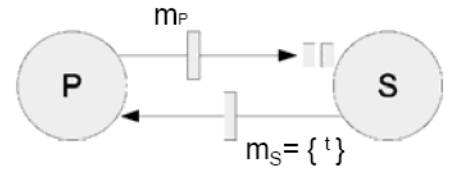
\includegraphics[width=0.5\textwidth]{resources/algoritmo_cristian.png}
                \caption{Solicitud de tiempo UTC mediante el algoritmo de Cristian}
                \label{algoritmo_cristian}
            \end{figure}

            El algoritmo sigue los siguientes pasos:

            \begin{itemize}
                \item En primer lugar, un proceso o máquina $P$, solicita el tiempo a un 
                servidor $S$, mediante un mensaje $M_p$. 
                \item $S$ devuelve la respuesta a $P$ incluyendo el tiempo $t$ en el mensaje 
                de respuesta $M_s$.
                \item Al recibir el mensaje, $P$ ajusta su tiempo añadiendo el tiempo transcurrido 
                entre el envío y la recepción (tiempo de transferencia o $Ttrans$), mediante la fórmula: 
                \[Reloj = t + Ttrans\]
            \end{itemize}
    
            Existe un tiempo de petición, un tiempo de respuesta, y un tiempo denominado de interrupciones 
            que comprende desde que llega el mensaje de solicitud del tiempo hasta que se envía una 
            respuesta con el nuevo tiempo.

            El tiempo de transmisión de un mensaje es $T_1-T_0 / 2$. El tiempo total de transmisión más 
            elaboración del mensaje de respuesta sería entonces $(T_1-T_0-I) / 2$, siendo $I$ el tiempo 
            de interrupciones (véase figura \ref{algoritmo_cristian00}). 

            \begin{figure}[htp]
                \centering
                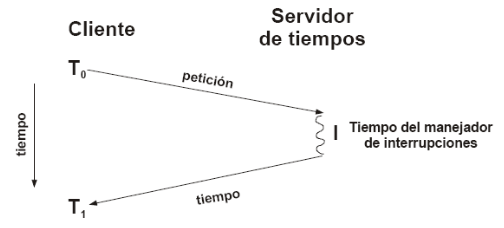
\includegraphics[width=0.5\textwidth]{resources/algoritmo_cristian00.png}
                \caption{Esquema del algoritmo de Cristian}
                \label{algoritmo_cristian00}
            \end{figure}

            De tal forma que el valor que se envía desde el servidor $S$ a $P$ se debe incrementar en 
            $(T_1-T_0-I) / 2$ para que pueda ser una estimación más realista.

            A pesar de su simplicidad, el algoritmo de Cristian ofrece varios problemas:

            \begin{itemize}
                \item El sistema puede estar muy centralizado en un servidor que transmite el tiempo 
                a los demás. Si dicho servidor se colapsa o se cae, se crea un problema de sincronización 
                en la red. Para solucionarlo se requerirán varios servidores que lleven a cabo esta 
                función, con la correspondiente coordinación de tiempo entre ellos.
                \item Si por casualidad se infiltrara un servidor S falso en el sistema, podría producir 
                unos daños bastante grandes, sobre todo en sistemas que manejen aplicaciones bancarias. 
                Para solucionarlo se necesitan procesos de autenticación del servidor, lo que aumenta el 
                tiempo de sincronización
            \end{itemize}

        \subsubsection{Algoritmo de Berkeley}

            Se procede a elegir un coordinador el cual tendrá el rol de maestro o lo que será lo mismo 
            de servidor de tiempo. El coordinador en este algoritmo en diferencia con otros algoritmos 
            de sincronización como es el caso del algoritmo de Cristian, no se mantendrá pasivo, se 
            encargará de solicitar la hora del resto de equipos, los cuales tienen un rol de esclavos, 
            dicha solicitud de hora se realizará de una forma periódica.

            Una vez los esclavos hayan respondido con su hora local, el maestro realiza una estimación 
            media de los retardos con los tiempos recibidos en los mensajes con cada uno de los equipos 
            esclavos, obteniendo así un tiempo medio que relaciona las horas recibidas durante la 
            solicitud y la hora propia del maestro.
            
            Realizada dicha estimación, el siguiente paso será actualizar los relojes de los equipos 
            esclavos. Para ello, el maestro enviará a cada esclavo el desfase que tiene respecto a la 
            hora promedio que se ha calculado. Se envía el desfase en lugar de enviar la hora coordinada 
            puesto que se debe tener en cuenta el error que aparecería por el tiempo de transmisión. 
            Finalmente, cada equipo se limitará a actualizar su reloj adelantándolo en caso de ir con 
            retraso o atrasándolo en caso de ir adelantado para aplicar la deriva recibida.
        
            \begin{figure}[htp]
                \centering
                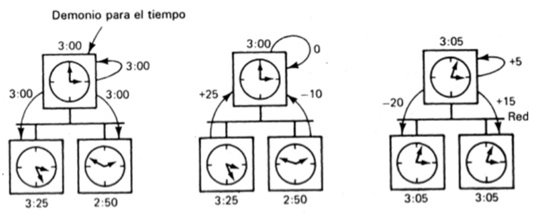
\includegraphics[width=0.8\textwidth]{resources/algoritmo_berkeley.png}
                \caption{Esquema del algoritmo de Berkeley}
                \label{algoritmo_berkeley}
            \end{figure}

            Estudiando dicho algoritmo se puede pensar que no se tiene en cuenta el tiempo de propagación 
            en la respuesta a la solicitud de la hora del esclavo a nuestro coordinador y por tanto, se 
            recibe una hora con retraso. Dicha situación no es un escenario que se necesite tener en 
            cuenta, puesto que la finalidad del algoritmo es la de calcular una hora promedio entre las 
            que se reciben con el sondeo del maestro a todos sus esclavos. Además, en una red de área 
            local entre los tiempos de propagación de mensajes entre maestro y los esclavos será 
            despreciable y, por ello, no es necesario tener en cuenta.

            El algoritmo de Berkeley realiza un promedio tolerante a fallos usando de base los tiempos 
            enviados por los esclavos, lo cual significa que únicamente se toman para calcular el promedio 
            los tiempos enviados por aquellos relojes cuya diferencia no difiere entre sí entre unos 
            umbrales estipulados, de forma que se entenderá que el resto de relojes no están funcionando 
            correctamente.

            En caso de fallo del maestro el proceso será el de elegir otro coordinador. Como fallo se 
            entenderá que el maestro no realice las solicitudes de tiempo periódicas, no envíe a cada 
            esclavo la deriva pertinente su reloj o simplemente que dote a los esclavos de un valor de 
            deriva el cual no es muy lógico. 

        \subsubsection{Protocolo de tiempo de red}

    \subsection{Sistemas basados en relojes lógicos}

        \subsubsection{Algoritmo de Lamport}

        \subsubsection{Relojes vectoriales de Mattern y de Fidge}

        \subsubsection{Protocolo BBS (Birman, Schiper, Stephenson)}

        \subsubsection{Relojes matriciales}

\section{Sincronización distribuida}

    \subsection{Algoritmos de elección y cooperación}

        \subsubsection{Algoritmo del matón}

        \subsubsection{Algoritmo del anillo}

        \subsubsection{Algoritmo de invitación}

    \subsection{Algoritmos de sincronización de procesos}

        \subsubsection{Algoritmo de exclusión mutua centralizada}

        \subsubsection{Algoritmo del testigo (\textit{token ring})}

        \subsubsection{Algoritmo de Ricart y Agrawala}

        \subsubsection{Algoritmo de Lamport}

        \subsubsection{Algoritmo de Maekawa}

        \subsubsection{Algoritmo descentralizado}

% BIBLIOGRAFÍA Y REFERENCIAS
\newpage
\begin{thebibliography}{X}
    \bibitem{} Desarrollo de un sistema expertocon lógica difusa, Jorge Franco Herrera y Angélica Franco Arias \\ \url{https://ingsistycomp.files.wordpress.com/2017/09/proyecto-1-sistema-experto-difuso.pdf}
    \bibitem{} Diseño de un Sistema Experto Difuso para la Determinación de la Densidad de Corriente en una Planta de Cromado, Carolina V. Ponce y Bayron Rojas \\ \url{https://scielo.conicyt.cl/scielo.php?script=sci_arttext&pid=S0718-07642019000200157}
    \bibitem{} Modelo basado en Lógica Difusa para el Diagnóstico Cognitivo del Estudiante \\ \url{https://scielo.conicyt.cl/scielo.php?script=sci_arttext&pid=S0718-50062012000100003}
    \bibitem{} Sistemas Expertos y Lógica Difusa \\ \url{http://catarina.udlap.mx/u_dl_a/tales/documentos/lmt/maza_c_ac/capitulo2.pdf}
    \bibitem{} Sistema de Control Difuso para Unidades de Cuidados Intensivos (UCI), Jefferson Steven Soto Medellín \\ \url{https://repository.ucatolica.edu.co/bitstream/10983/1278/1/Sistemas%20de%20Control%20Difuso%20para%20Unidades%20de%20Cuidado%20Intensivo%20(Trabajo%20Final)%20701429%20Nuevo.pdf}
\end{thebibliography}

\end{document}
